\subsection{Interruttore crepuscolare}

Nell'ultima parte dell'esperienza abbiamo assemblato un interruttore crepuscolare, cioè un circuito elettronico che alimenta un carico (LED) in condizioni di bassa luminosità ambientale e interrompe l'alimentazione in condizioni di alta luminosità ambientale.

\begin{figure}[ht]
 \centering
   {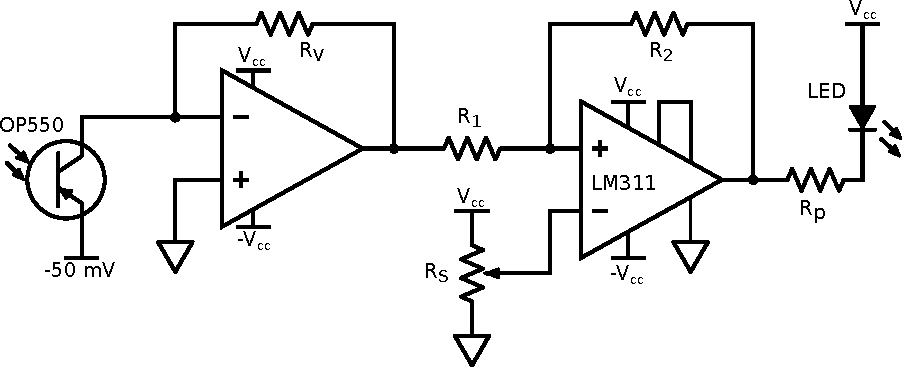
\includegraphics[width=12.5cm]{../E04/latex/c_crepuscolare.pdf}}
 \caption{Circuito dell'interruttore crepuscolare. Come vediamo chiaramente, la parte con l'op-amp $\mu$A741 è un semplice amplificatore in tensione ($R_F = \SI{1}{\Mohm}$) La seconda parte del circuito è un comparatore con isteresi, settata dal rapporto $R_1/R_2$ ($R_1 = \SI{50}{\kohm}$ e $R_2 = \SI{100}{\kohm}$). La tensione di riferimento deve essere scelta in modo da decidere con quanta luminosità si vuole che l'interruttore scatti. Per far ciò abbiamo usato un partitore utilizzando un trimmer ($R_S$) da \SI{10}{\kohm}. La resistenza di pull-up è stata scelta di  \SI{1}{\kohm}, così da avere una corrente sufficiente per far accendere il led.}
 \label{cir4:crepuscolare}
\end{figure}

Un circuito di questo tipo necessità di almeno due componenti: il sensore di luminosità (fototransistor OP550) che fornisce la variabile circuitale collegata alla luminosità ambientale e un blocco di comparazione che \textit{decide} se alimentare o meno il carico confrontando il segnale dato dal primo blocco con un segnale di riferimento.

Il componente principale del primo blocco è il fototransistor OP550 che agisce come una sorgente di corrente, generando una corrente dell'ordine del \si{\uA} se esposto alla luce.
Tale corrente è però difficilmente manipolabile, pertanto abbiamo deciso di utilizzare un convertitore corrente-tensione per trasformare e amplificare il segnale in modo tale da poter essere utilizzata come segnale di ingresso del secondo blocco.

Un convertitore corrente-tensione può essere implementato facilmente utilizzando un opamp $\mu$A741 in modalità di amplificatore invertente con retroazione negativa (vedi Figura \ref{cir4:crepuscolare}).
In questo modo, la tensione in uscita dell'opamp sarà legata alla corrente che attraversa il sensore dalla seguente equazione:

\begin{equation}
	V_{out} = R_F \,\, I_{OP550}
\end{equation}
dove $R_F$ è la resistenza posta sul ramo di retroazione (nel nostro caso $R_F = \SI{1}{\Mohm}$) e $I_{OP550}$ è il modulo della corrente passante nel fototransistor.

Il secondo blocco del circuito è invece composto da un opamp LM311 utilizzato come comparatore con isteresi (o trigger di Schmitt).
Sul ramo di retroazione e tra il terminale positivo e l'ingresso del segnale - che corrisponde all'uscita dell'opamp $\mu$A741 - sono state poste due resistenze per creare l'isteresi affinché eventuali rumori di fondo non disturbassero il funzionamento del circuito.
Nel nostro caso abbiamo utilizzato due resistenze $R_1 =$ \SI{5}{\kohm} e $R_2=$ \SI{100}{\kohm} in modo da avere un ampio margine di sicurezza.

Come si può notare dal grafico in Figura \ref{gr4:neon} il rumore ambientale dato dalle lampade al neon ha una forma d'onda sinusoidale di frequenza \SI{100}{\hertz} e ampiezza picco-picco \SI{80}{\mV}, pertanto sarebbe stata sufficiente un'isteresi di appena $\frac{V_{CC}}{100} \approx \SI{150}{\mV}$

Per impostare la tensione di soglia, invece, abbiamo creato un partitore collegando i due connettori esterni di un trimmer resistivo da \SI{10}{\kohm} a +\SI{15}{\V} e a comune, mentre abbiamo collegato il terminale centrale del trimmer all'ingresso invertente del LM311.
In questo modo potevamo scegliere la tensione di soglia girando semplicemente un cacciavite.

Infine abbiamo posto il carico da alimentare tra l'alimentazione positiva +\SI{15}{\V} e la resistenza di pull-up ($R_P=$ \SI{1}{\kohm}).

\begin{figure}[ht]
 \centering
   {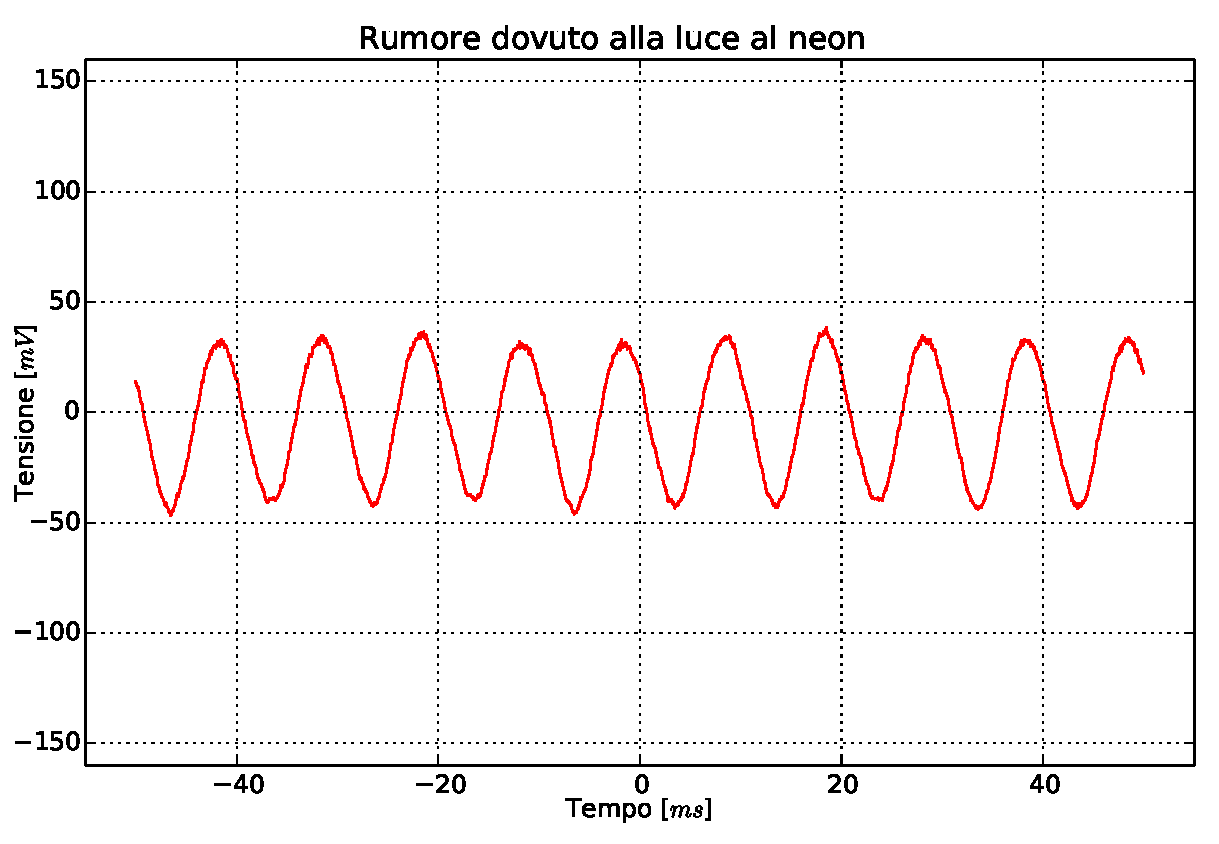
\includegraphics[width=14.5cm]{../E04/latex/neon.pdf}}
 \caption{Rumore ambientale determinato dalla luce delle lampade al neon del laboratorio incidente sul fototransistor e amplificato dall'opamp $\mu$A741. I dati sono stati ricavati separando i due blocchi del circuito e misurando la tensione all'uscita dell'opamp $\mu$A741.}
 \label{gr4:neon}
\end{figure}
